% E.5 △ABC, AB=6, ∠BAC=45°. BD 角平分线 (D on AC). M∈BD, N∈AB.
% A(0,0), B(6,0). ∠BAC=45° → C 在射线方向 (cos45°, sin45°). 取 C=(8cos45°, 8sin45°)=(5.66,5.66)
% BD 角平分线: ∠ABC 平分, 我们先估 ∠ABC. 用 A=(0,0), B=(6,0), C=(5.66,5.66)
% AC方向 (cos45°,sin45°). BC = C-B = (-0.34, 5.66), |BC|≈5.67
% 简化: 取 △ABC 中 D 大致位置, 示意图即可
\documentclass[tikz,border=4pt]{standalone}
\usepackage{ctex}
\usepackage{amsmath}
\usetikzlibrary{calc}
\begin{document}
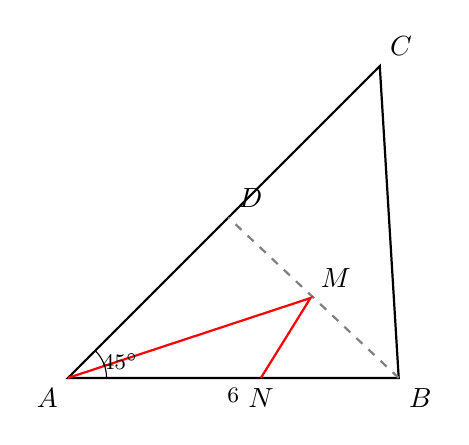
\begin{tikzpicture}[scale=0.7, thick]
  \coordinate (A) at (0,0);
  \coordinate (B) at (6,0);
  \coordinate (C) at (5.6569, 5.6569);  % AC=8 along 45°
  % BD 角平分线交 AC. 角平分线公式: D 分 AC 使 AD/DC = AB/BC.
  % AB=6, BC=√((-0.343)^2+5.657^2)=√(0.118+32.0)=5.667
  % AD/DC = 6/5.667 → AD = 8·6/(6+5.667) = 4.114
  \coordinate (D) at (2.910, 2.910);
  \coordinate (M) at (4.4, 1.45);   % M on BD
  \coordinate (N) at (3.5, 0);     % N on AB

  \draw (A)--(B)--(C)--cycle;
  \draw[gray, dashed] (B)--(D);
  \draw[red, thick] (A)--(M)--(N);

  % 标 45°
  \draw[thin] (0.7,0) arc[start angle=0, end angle=45, radius=0.7];
  \node[font=\footnotesize] at (0.95, 0.3) {$45^\circ$};

  \node[below left] at (A) {$A$};
  \node[below right] at (B) {$B$};
  \node[above right] at (C) {$C$};
  \node[above right] at (D) {$D$};
  \node[above right] at (M) {$M$};
  \node[below] at (N) {$N$};

  \node[below, font=\footnotesize] at ($(A)!0.5!(B)$) {$6$};
\end{tikzpicture}
\end{document}
